\chapter{Results}
\todo{By results, do we limit ourselves to the usability tests? If not we need to change this opening text. /H}
Results can be presented in different ways. One way would be to describe the usability tests in detail, and another way would be to only summarize the results in table. 
By describing all usability tests in detail, it would be hard to get a good overall view of the findings. Focusing more on something also means focusing less on something 
else, and there are other parts of the documentation that deserve that attention more. It would therefore not be ideal to do lengthy elaborations on each teaching material.
On the flip side, only giving a summary on the findings would leave out describing the crucial process. The process mainly includes:
\begin{enumerate}
	\item Performing a usability test
	\item Identifying what can be learned from the data
	\item Figuring out how the particular teaching material can be improved from the data
	\item Revising the teaching material (preferably in an effective manner)
\end{enumerate}
The ideal way of delivering the results should entail a comporomise between these two extremes. The finding has therefore been divided into a sample case and a summary.
The sample case describes a teaching material thouroughly, delving into details of the process and findings, exemplifying the usability testing process. 

\section{Summary of usability tests}

Seen in table \ref{table:testsummary} is a summary of all the usability tests. Each test has a codename containing one lower case letter, referring to the material that was tested, and an uppercase letter, referring to the test subject. For example, test "nB" tested material "Nätverk - insamling av data" on test subject B. 

Every test subject also has a longer codename containing their age, profession and teaching experience. This is according to section \ref{subjectanonymity}, about what information is disclosed about the test subjects. The format of this codename is as follows:

\begin{itemize}
  \item A letter in alphabetical order chosen chronologically. For example, test subject "B" was done earlier than test "D" but later than test "A".
  \item The age of the test subject, rounded to the nearest 25 years.
  \item The letter "T" if they worked or had worked as a teacher, or "S" if they were studying teaching.
  \item The total number of years they worked as a teacher, rounded up if less than 10, otherwise rounded to the nearest 5 years.
\end{itemize}

Thus, "A30T2" means test subject A is approximately 30 years old, has worked as a teacher, and has approximately two years of teaching experience.

\bgroup
\def\arraystretch{1.5}
\begin{table}[H]
\centering
\caption{Summary of all usability tests of the study}
  \begin{tabular}{p{3cm}p{2.5cm}p{5cm}p{2.5cm}} \hline\hline
  Test codename & Date for test & Material that was tested & Test subject \\ \hline
  mA & 2018-04-24 & Mönster och talföljder - Pascals triangel ur slantsingling & A30T2 \\ \hline
  nB & 2018-04-30 & Nätverk - insamling av data & B25S \\ \hline
  lC & 2018-05-03 & Vad ska lotten kosta? & C35T3 \\ \hline
  aD & 2018-05-09 & Konsten att bestämma arean & D35T6 \\ \hline
  sE & 2018-05-09 & Område statistik & E40T4 \\ \hline
  oF & 2018-05-14 & Modellering & F50T30 \\ \hline
  nF & 2018-05-14 & Nätverk - insamling av data & F50T30 \\ \hline
  mG & 2018-05-24 & Mönster och talföljder - Pascals triangel ur slantsingling & G25T2 \\ \hline
  dG & 2018-05-24 & Den dolda och tvetydiga matematiken & G25T2 \\ \hline
  dH & 2018-05-30 & Den dolda och tvetydiga matematiken & H25S \\ \hline
  dI & 2018-06-12 & Den dolda och tvetydiga matematiken & I30T1
  \\ \hline\hline
\end{tabular}
\label{table:testsummary}
\end{table}
\egroup

\section{Sample case 1. Kleinmaterial: Nätverk} \label{samplecase1}
Each teaching material tested has a different story to tell. Keep in mind that some of the content of the steps below are common to all teaching materials tested, while some are specific to the particular teaching material.

\subsection{The preexisting work}
The sample teaching material was produced by a team at Kleindagarna. These consisted of a handful of teachers, a subject expert and a Klein-representative. When the workshop at Kleindagarna was over, the teaching material was published on Kleindagarna's website. 

\subsection{Usability test I}
The first usability test was performed by one of the authors of this report on the other author. As this was the second ever usability test performed, the intention was primarily to identify what to take into account for future usability testing and to identify the possibility of improving the usability testing methodology. The method consisted of following a script document on a computer including:
\begin{itemize}
    \item A table made to be filled with personal information
    \item A list of keywords and questions (manuscript) inspired by the usability test script created by Steve Krug.
\end{itemize}

Results from this test included:
\begin{itemize}
    \item Unclear if some tasks were meant to be executed by teacher or students.
    \item The material expected the teacher to be very familiar with the subject, tackling advanced areas of mathematics with mostly bullet points, expecting the teacher to provide the explanation.
    \item There was a concern on the material having too large scope. The material includes network theory, statistics, algorithms and data protection laws (GDPR), and aims to both explain and problematize all of these aspects.
\end{itemize}
\subsection{Revision of methodology}
After usability testing the teaching material, the authors identified that there was very limited information presented in the list of teaching materials on Kleindagarna's website. This made it difficult for the curious to know if the material was suitable for them. Because of that, a new list of teaching materials was compiled. This consisted of information not just what the subject of the material was, but also for what grade it was suited and a more detailed description of the teaching material.\\
After the usability test, a discussion arose on what type of material the revisions would be. Two suggested possibilities were documents (i.e. pdf- or odt-files) and presentations (e.g. pptx-files). A document would have the strength of being easily skimmed and modified. A presentation would have the strength of being a ready-made lesson material, with the potential of not requiring as much planning time. The discussion culminated in the decision to choose type on a case-by-case basis. Some factors to take into account when deciding on the type would be: results from usability tests, perceived intent of original creators and what form would be most suited for the particular teaching material.
\subsection{Watching the Klein-lecture}
Before designing a teaching material, the participators on Kleindagarna receive a lecture by the subject-expert. This lecture was recorded and confidentially shared online. Before revising the material, it was decided that it would be beneficial to watch this lecture, to learn more about the theory the material was based upon and what the creators intended the students would learn.
\subsection{Usability test II}
The same revision was tested again. The test subject this time was a Klein-representative that had been involved in the creation of the original teaching material. Testing teaching materials on a subject that was not a teacher in upper-secondary-school or a teacher student aiming to teach at upper-secondary-school was not the norm. One purpose of this was to analyze how rewarding usability testing non-intended subject could be. The test subject is also teaching mathematics on an upper-secondary-school level, but to post-secondary school students (one additional difference is that the pace of the courses are comparably higher than in upper-secondary-school). Results from this test included:
\begin{itemize}
    \item The teaching material wasn't considered complete by the creators.
    \item The biggest remaining problem of the material design lies in a student activity where the class are to compile data to create a network. To be able to make the network and its analysis meaningful, it was suggested that the compiled data should be personal and able to lead to a finding. Ultimately, the activity asks for generated data, instead of personal, more valuable data. The reason for this is because no conceivable alternative could eliminate the risk that personal data could result in undesirable findings. For example if the data collected answers what students had lunch together, outcasts are visible in the finding.
\end{itemize}
\subsection{Revision of teaching material}
From the data collected, the following revisions were made:
A decision was made to revise the material in the form of a presentation, with the aim to offer a ready-made presentation with enough explanation of the required theory to be a desirable product. To realize this, changes were made to the structure and to content.
\subsubsection*{Structural changes}
\begin{itemize}
    \item The separation of information to the teacher and the main presentation was improved by implementing tabs similar to how many websites function (see figure~\ref{tabs}). This also clarified the structure to the user, enabling the user to quickly get an overview of the structure.
    \item The presentation's first slides contain useful information targeted to a curious teacher including how to read the important presentation notes (as these consists of teacher instructions and explanations). Previously, the first slide contained information on who had created the presentation. As this information was deemed less important than what the presentation actually encompassed, this slide was moved to the end of the presentation instead.
\end{itemize}

\begin{figure}[H]
\centering
%
\includegraphics[width=\linewidth]{figure/tabs1.png}

\includegraphics[width=\linewidth]{figure/tabs2.png}
\caption{Tabs were introduced to give an overview of the material.}
\label{tabs}
\end{figure}

\subsubsection*{Content changes}
\begin{itemize}
    \item As mentioned previously, the presentation contains teacher instructions and explanations in the form of presentation notes. These can be printed or read in the presentation program, and also viewed while presenting (see figure~\ref{notes}). This was previously missing from the teacher material, or carelessly intertwined with content that seemed to be aimed to students.
    \item Activities were altered to be either less vague or more closely tied to what the students are expected to learn.
    \item The content was modified to be easily understood and conveyed. An example of this was replacing the headings so that they describe their respective slide, instead of being named after the current 5E-phase.
\end{itemize}

\begin{figure}[H]
\centering
\frame{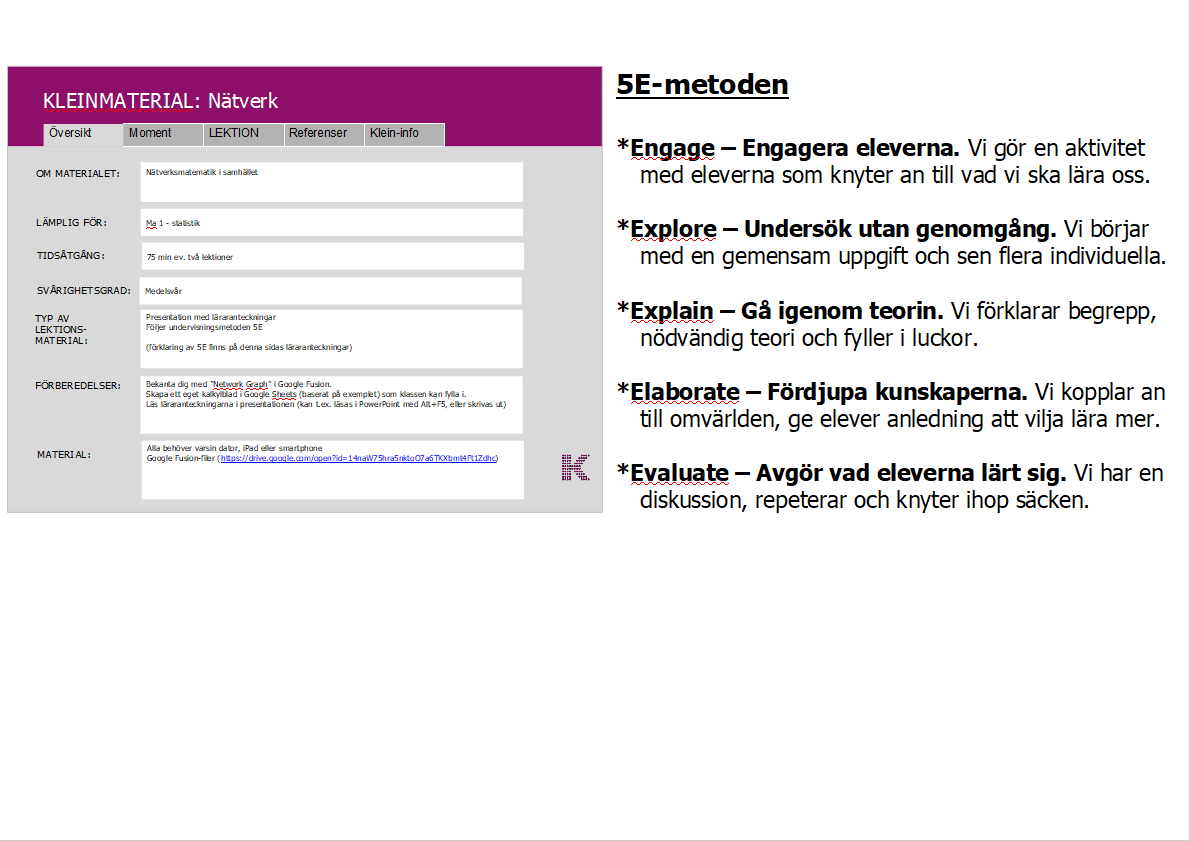
\includegraphics[width=\linewidth]{figure/notes.png}}
\caption{Presentation notes were introduced, to separate content aimed at teachers from content aimed at students.}
\label{notes}
\end{figure}

\subsection{What was learned from this case?}
From this particular case, the following knowledge was obtained:
\begin{itemize}
    \item Someone involved in the creation of a teaching material can have a very different experience and connection to the teaching material than what is conveyed to a reader. Maybe there is a part the creator is not satisfied with, but the reader might assume it is meant to be complete and only understand it as poorly made. This exemplifies the flaws of one-way communication.
    \item There needs to be a decision on how the teaching material is presented and what it aims to be. It can be everything from inspiring reading material to a documentary.
\end{itemize}

\section{Sample case 2. Kleinmaterial: Vanliga missuppfattningar} \label{samplecase2}

\subsection{The preexisting work}

Just like sample case 1, in section \ref{samplecase1}, the teaching material in sample case 2 was produced by a team at Kleindagarna. It was about common misconceptions in mathematics. It had a list of exercises in the beginning and a list of correct answers in the end. In between these lists, it had a lesson plan. One of the main points of the material was to categorize different mathematical exercises as "beräkning" (calculation), "förenkling" (simplification), and "ekvationslösning" (equation solving).

[FIGURE: MATERIAL ZOOMED OUT]
[REFERENCE: MATERIAL APPENDIX]

\subsection{Usability tests and problems found}

There were three relatively similar usability tests done on this material. The tests revealed that the material had some problems with structure and explaining what the exercises were supposed to teach. All subjects understood the main points of the material eventually, but it took them a while to dos o. In order of the tests done, these problems were found:

\begin{itemize}
  \item In test dG, see table \ref{table:testsummary}, the meaning of the different categories were unclear at first. The test subject first thought the exercises were examples of solutions rather than exercises. The subject also expressed that it took a lot of scrolling up and down to connect the first list with the lesson plan.
  \item The test subject in test dH expressed directly that they wanted a written purpose, connection to the curriculum, and time estimations. They expressed a need for more descriptions in general since the material was lacking an introduction or background, though they did not want too much text either.
  \item In test dI, the test subject scanned the text up and down more compared to the previous tests, rather than reading it from top to bottom. This time, it took even longer for the subject to understand the material. This revealed a possible problem with the material's adaption to scanning. For example, the material had headings called things such as "Part A" and "B:2", which did not explain what the different parts were about. Furthermore, starting the material with a list might have meant that the subject did not know where to start reading, similarly to what happened in tests dG and dH.
\end{itemize}

\subsection{Lessons learned}

Since three test subjects chose to test this material and revision, it proved to be a good chance to study how different subjects react to the same material. According to Krug (2010), testing the same thing several times tends to reveal the same problems, aside from a couple of differences. This was found to be the case with this material; the unclear structure and lack of introduction was prominent in all tests, but the subjects read the material differently. While in dG and dH the subjects read the material more in-depth, in dI they used more of a scanning approach. This likely affected their abilities to understand the material. The most important lesson gained from this, however, was that test subjects do read the same material in different ways, possibly due to different reading habits in general. This is further strengthened by another test, aD, in which the teacher tended to read everything top-to-bottom and in-depth directly, including the list of materials.

Interestingly, despite complaining about the material's clarity, all test subjects found a way that they could hypothetically use the material in a lesson, and two of them expressed positive thoughts about the material. More specifically, dH said that the material was "fun, with a lot of interactive parts" and "you can cut out [the exercises] and hold the lesson directly, which is good." In dG, the subject said that the material "feels very fun and doable", and "a fun way for the students to get a bit of a [habit]." This might point toward that a material which is difficult to understand still can be useful, if the rest of its content is good and relevant enough.

\section{The materials list}

The original list of materials was remade and revised continuously after feedback from the usability tests. It proved useful as a way to study how the teachers picked their materials, and what information they want when doing so. Below is presented the original list made by Kleindagarna, and the revised list made as part of this thesis.

\subsection{The original materials list}

The original list of materials was a part of Kleindagarna's website. This list contained information about the "Kleinföreläsare" (Klein lecturer), generic maths subject, who was testing the material, followed by a link to most of these materials in PDF-format. This information did not prove enough for the test subjects looking through the materials, which might be due to Kleindagarna's website being designed for a different target group. Note that the design of Kleindagarna's list seen in figure \ref{fig:originmaterialslist} was changed slightly during the thesis, and thus the revised list of materials was based on a slightly different design. However, the change only affected the color and font, and the information in the list remained unchanged. Thus, this change should have little to no effect on the comparability between these different lists.

\begin{figure}[H]
\centering
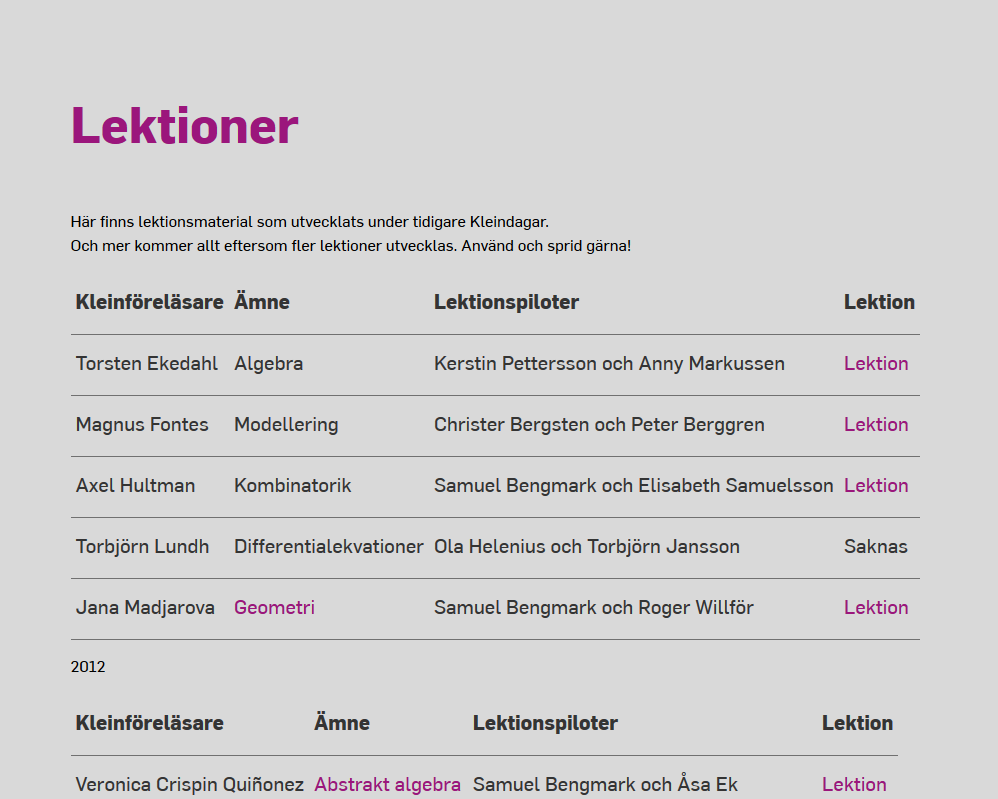
\includegraphics[width=\linewidth]{figure/screenshot_materiallista_kleindagarna.png}
  \caption{The original list of materials on Kleindagarna's official website [KÄLLA: KLEINDAGARNA.SE, LEKTIONSSIDAN].}
\label{fig:originmaterialslist}
\end{figure}

\subsection{Revisions of the materials list}

Revisions of the list of materials were made continuously during the project, building on feedback from the usability tests. The list was remade from scratch in the form of a website, similar to the original list but containing other information, see figure \ref{fig:revmaterialslist}. Comparing the original list with the revised list, a couple of things were changed:
\begin{itemize}
	\item A tagline was added under the title: "Lektionsplaneringar med nya matteperspektiv" in Swedish, or "Lesson plans with new mathematical perspectives" in English. This was meant to change the expectations of the teachers looking through the list, so they knew the materials were about mathematics, and that they had innovative perspectives on mathematics rather than remaking typical maths lesson materials.
	\item A description was added for every material due to teachers expressing during the tests that they wanted to know more about the material they were going to choose. The descriptions were originally taken directly from the materials and slightly reworked, leading to some materials lacking a description due to not having one in the material itself. This further lead to teachers ignoring the materials that were lacking a description during some tests. Thus, descriptions were added to all the materials.
	\item The "Lektionspiloter" and "Kleinföreläsare" parts of the list were removed since few of the test subjects would understand what it was or know the people by name, and more space was needed for other information.
	\item "Relevant(a) gymnasiekurs(er)", in English "Revelant secondary school course(s)", were added due to them existing in most of the materials themselves, and thus easily added into the list. Likewise, "Koppling till ämnesplan", "Connection to the subject curriculum" in English, was added in the same way, also replacing "Ämne" in the original list..
	\item A title was added to every material in the list to make the materials more scannable instead of having to read the whole description to understand the general idea of the material.
\end{itemize}

\begin{figure}[H]
\centering
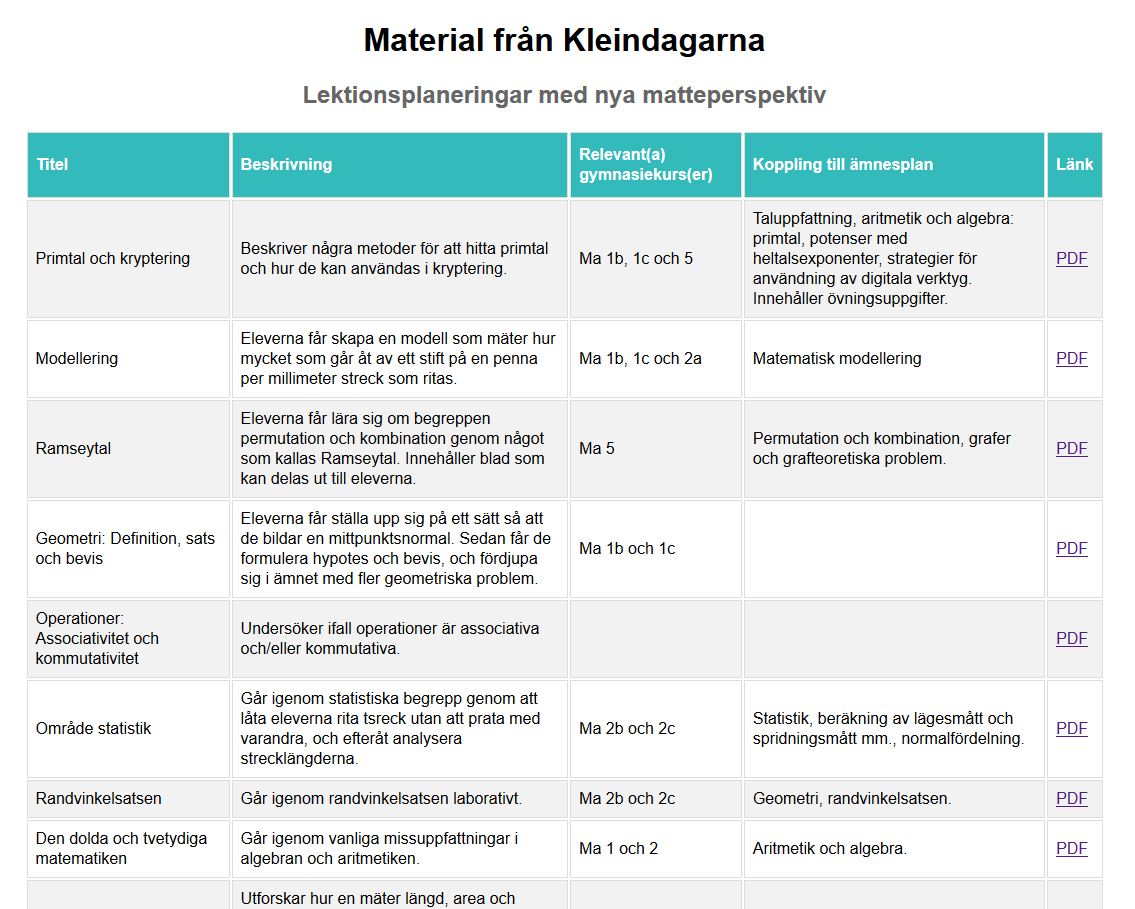
\includegraphics[width=\linewidth]{figure/screenshot_materiallista_revision_2.png}
  \caption{The second revision of the list of materials, based on Kleindagarna's original seen in figure \ref{fig:originmaterialslist}.}
  \label{fig:revmaterialslist}
\end{figure}

\subsection{Results from studying how teachers chose their materials} \label{pickmaterials}

Studying how the teachers chose one material from the materials list generated a few findings that might point toward how teachers choose materials in general. This is relevant for discussing obtainability later in the report.

One common finding was that the teachers want to know what type of material they are picking. For example, they want to know whether the material is a practical lab kind of lesson, or if it is a more common combination of lecture and exercises. Information about the material's connection to the curriculum, and what courses it can be used in, was also appreciated by the test subjects.

Another finding was that teachers looked for materials that connected to what they were teaching at the moment. For example, in test sE, the teacher chose the statistics material to get some perspective on what they had taught recently. This is important to consider in the case of innovative or different materials, since teachers might ignore such materials in favor of those that connect more strongly to their teaching curriculum.

Important to note about these findings is that the teachers were told to choose one material per test, without opening it. Thus, they did not learn anything about the materials other than what was shown in the list of materials. This is different from reality, since if a teacher would visit a website containing several materials, they would be able to open each of them and look them over before picking one that they'd use in a lesson. However, the findings in this study might still be useful for getting some pointers in what teachers are looking for in a material, and what they want to know about it.

\section{General perspective: Things that were learned from all the usability tests}
The previous usability test cases in this chapter described how results were produced from a couple of specific tests. In a similar manner, more results were produced by going through the tests one by one and summarizing the findings, and comparing the tests next to each other. Below are some findings from this general analysis.

\subsection{Comparisons between the teachers' typical lessons}
Part of the usability test consisted of asking the teachers what their typical lesson looked like. The answers the teachers gave showed that most teachers work with a combination of lectures in group and individual student exercises, even if their lesson lengths and structures were different. For example, one teacher had three hour lessons with multiple 10 minute breaks, while another had one hour lessons. Other than that, tools such as Goegebra, calculators, computers, and online quiz tools were mentioned by some individual teachers.

\subsection{Making the material intuitive for different behaviours is important}
Because of the difference in how teachers read a material, where one might instantly read the material in-depth and the other might just scroll down while scanning it, having a material be intuitive at first glance is a good thing. Some materials took the teachers a while to understand, which could have been rectified through a more clear structure and by following typical patterns that the teachers are used to. One pattern that was asked for directly in two of the usability tests (dH and dI) was to have an introductory text, which was lacking for the specific material that was tested. At the same time, in one of the tests (mA), the teacher completely ignored the introduction at first to make sense of the material's content by itself. In either case, the material should ideally be clear to understand for both types of material reading behaviours.

\subsection{Having student handouts as part of a material is appreciated} \label{handouts}
All materials did not have parts that could be handed out to students, such as a list of exercises. However, many teachers seemed to appreciate such "handouts", or ask for them when they were missing. For example, one teacher, in test aD, wanted a handout for the student that explained a difficult word that they hadn't encountered before. Another teacher said in test dI that they could use a list of exercises by itself without following the exact lesson plan. This shows that exercises as a part of a material can improve the adaptability of the material. In contrast to this, in test nB one teacher expressed that materials can also work as a source of inspiration rather than something concrete and finished as a handout or a finished lesson plan. An important aspect of both of these materials, the "concrete handout" and the "source of inspiration", is the amount of work that these different types require for adaption into a real lesson: The handout can be printed and handed out directly, while the inspiration has to be reworked into a new material.

\subsection{Accounting for teachers' and students' previous knowledge} \label{prevknowledge}
A common problem among many materials was the teacher's lack of previous knowledge about the subject that the material presented. The most common and concrete problem that appeared was when new vocabulary was used, such as RSA (tests lC and dH) and Dido's problem (dH). There was also an issue with one teacher not feeling competent enough to teach a subject that a material covers (sE). In contrast, another teacher expressed that a material could be explored together with the students when the teacher did not know everything about it either (lC). Similarly, some materials seemed too difficult for certain teachers to use due to their students' lack of previous knowledge (aD and sE).

\subsection{Finding common usability problems}
In every test, at least one unclear explanation or structure, unanswered question, or other smaller, easily rectified usability problem was found. Thus, the usability tests proved effective in finding these problems. Examples of the problems found include:
\begin{itemize}
	\item No clear explanation about what part the student should do and what part the teacher should do during a lesson.
	\item A lack of description of the axes in a diagram.
	\item Mixed use of comma (,) and dot (.) as decimal separator.
	\item An undefined word that needed explanation (Galton board).
	\item Unclear use of the 5E-structure when it was not used as the teacher expected it to be used.
	\item Unclear whether "degrees" was referencing temperature, geometric angles, or "levels."
	\item Misunderstandings about what a list of exercises was, where the teacher described it simply as a "list" of unknown purpose.
	\item Instructions that required more explanation. In this case, the instructions merely showed a couple of numbers without describing what the numbers were for; "0,0,0,50...", where it was explaining a point system for gambling with dice.
\end{itemize}

Although many of these misconceptions were often understood by the test subject after a while, it often took a lot of time, and likely frustration, for them to figure it out.
